\chapter{Sim-to-Real Deployment}
\label{ch:sim_to_real}

\section{Overview}

The preceding chapters developed and evaluated an articulated tractor-trailer controller entirely within a 2D simulation environment. This chapter describes the transfer of that controller to a physical robotic platform, constituting the sim-to-real component of this thesis. Unlike a conventional model-based stack, the deployed system does not re-implement a hand-derived tracking law on the vehicle. Instead, the simulation-trained reinforcement-learning (RL) policies are executed directly on hardware through a thin bridging layer that reproduces the observation and action interfaces the policies were trained against. The objective is to demonstrate that the vehicle model, the observation definitions, and the learned control logic established in simulation can be ported to real hardware with minimal algorithmic redesign, and to characterize the engineering challenges encountered during that transfer.

The deployment is built on a deliberately stripped-down Autoware stack. The standard Autoware localization and perception pipelines are retained essentially unchanged, while the behavior, planning, and control layers are replaced by a custom RL bridge that runs the forward and reverse policies. Two pieces of supporting infrastructure are described in detail because they are specific to the articulated, sensor-light platform: an onboard LiDAR-based hitch-angle estimator that recovers the articulation angle without any trailer-mounted sensor, and a Smith predictor~\cite{smith1957closer} that compensates for actuator delay so that delay-free-trained policies behave correctly on a lagging physical actuator.

\section{Hardware Platform}

\begin{figure}[t]
  \centering
  \safegraphic[width=0.85\textwidth]{figures/hardware/platform.jpg}{Photo of the AgileX Hunter SE tractor coupled to the lab trailer through the revolute hitch.}
  \caption{The physical articulated platform: an AgileX Hunter SE tractor coupled to the lab trailer through a revolute hitch at the tractor rear axle.}
  \label{fig:hw_platform}
\end{figure}

\subsection{Tractor Vehicle}

The physical tractor is an AgileX Hunter SE, a compact electric wheeled unmanned ground vehicle with an Ackermann steering geometry. The relevant mechanical parameters are a wheelbase of $0.65$\,m, a wheel radius of $0.15$\,m, and a maximum steering angle of $0.436$\,rad ($25^\circ$). Vehicle actuation is commanded over a CAN bus on a 20\,ms cycle. Speed commands are encoded as 16-bit signed integers in units of 1\,mm/s (the commanded speed in m/s scaled by $1000$) and steering commands as 16-bit signed integers scaled by approximately $1320$ counts per radian ($\approx 0.8$\,mrad per count).

\subsection{Trailer}

The trailer is coupled to the tractor through a revolute hitch joint located marginally behind the tractor rear axle, which was added to the tractor-trailer model used for training. The lab trailer has a wheelbase of approximately $2.8$\,m and a body width of roughly $0.33$\,m. The articulation angle $\gamma$, defined as the difference between the tractor and trailer headings ($\gamma = \psi_\text{truck} - \psi_\text{trailer}$), is estimated onboard from the tractor's own LiDAR rather than measured by any trailer-mounted sensor. The procedure is detailed in Section~\ref{sec:hitch_estimation}. The estimate is published to the ROS2 network on the \texttt{/vehicle/trailer\_state} topic. The control bridge consumes the most recent published value, with no staleness gating currently applied. Two distinct angular limits appear in the stack and should not be conflated. The onboard estimator clamps the published articulation estimate to $|\gamma| \le 90^\circ$, whereas the deployment trailer model defines a tighter operational limit of $|\gamma| \le 80^\circ$ ($1.40$\,rad), itself below the $90^\circ$ jackknife condition used to terminate simulation episodes.

\subsection{Sensor Suite}

\begin{figure}[t]
  \centering
  \safegraphic[width=0.85\textwidth]{figures/hardware/sensor_suite.jpg}{Photo of the onboard sensor suite mounted on the tractor.}
  \caption{Onboard sensor suite: the front-mounted RoboSense Helios LiDAR, the Basler cameras, the u-blox GNSS antenna, and the WitMotion IMU.}
  \label{fig:hw_sensors}
\end{figure}

The vehicle is instrumented with the following sensors:

\begin{itemize}
    \item \textbf{LiDAR}: RoboSense Helios mechanical LiDAR mounted at the front of the tractor, publishing 3D point clouds on \texttt{/rslidar\_points}. This single sensor is reused for three purposes: NDT-based localization~\cite{biber2003ndt}, environment perception, and onboard hitch-angle estimation.
    \item \textbf{Cameras}: Six Basler Pylon industrial cameras (rear, rear-right, center, left, merging, and right) producing compressed color images. The cameras are not consumed by the LiDAR-based RL policies and are used for logging and monitoring only.
    \item \textbf{IMU}: WitMotion 6-DoF inertial measurement unit, with a gyroscope-bias estimator applied in the localization pipeline.
    \item \textbf{GNSS}: u-blox ZED-F9P receiver with RTK corrections, providing centimeter-level position estimates converted to MGRS coordinates for Autoware localization.
    \item \textbf{Wheel odometry}: Vehicle speed and steering-angle feedback recovered from CAN messages and fused with IMU data for dead-reckoning between GNSS and scan-matching updates.
\end{itemize}

\section{Software Architecture}

\subsection{Middleware and Framework}

The deployment stack runs on ROS2 Humble (Ubuntu 22.04)~\cite{macenski2022ros2} and is integrated into the Autoware autonomous-driving framework~\cite{kato2018autoware}. Autoware provides modular localization, perception, planning, and control pipelines whose interfaces are defined by standardized ROS2 message types. As introduced in the overview, this deployment keeps the standard sensing, localization, and perception modules and replaces only the planning and control layers with the learned RL bridge.

\subsection{Relationship to the Conventional Articulated Pipeline}

For context, Autoware's conventional approach to articulated vehicles is fully model-based. A truck-trailer mode manager routes goals to a freespace planner (a hybrid A\textsuperscript{*} search~\cite{dolgov2010hybridastar} that respects the non-holonomic constraints of the articulated vehicle), and the resulting reference trajectory is tracked by a model-predictive or LQR lateral controller. This model-based pipeline exists within the wider project and represents the standard, well-understood baseline for trailer control. The relevant control background is reviewed in Chapter~\ref{ch:literature_review}. The contribution of this thesis, however, is the learned controller, and the deployment described here therefore routes control through the RL bridge instead of the planner/MPC chain. The two are mutually exclusive at run time and are selected at launch. \Cref{fig:autoware_stack} shows which modules are retained and which are replaced.

\begin{figure}[t]
  \centering
  \resizebox{\textwidth}{!}{\begin{tikzpicture}[
  >=Stealth, font=\footnotesize, node distance=8mm and 12mm,
  block/.style={draw, rounded corners, align=center, inner sep=4pt, minimum height=10mm, text width=20mm},
  lbl/.style={midway, font=\scriptsize}
]
  \node[block] (sens) {Sensing\\{\scriptsize LiDAR, GNSS, IMU}};
  \node[block, right=of sens] (loc) {Localization\\{\scriptsize (NDT)}};
  \node[block, right=of loc] (perc) {Perception};
  \node[block, right=of perc, fill=black!8] (rl) {RL bridge\\{\scriptsize TD3 policy}};
  \node[block, right=of rl] (veh) {Vehicle\\{\scriptsize Hunter SE}};

  \draw[->] (sens) -- (loc);
  \draw[->] (loc) -- (perc);
  \draw[->] (perc) -- (rl);
  \draw[->] (rl) -- (veh);

  % Autoware retained group
  \begin{scope}[on background layer]
    \node[draw, dashed, rounded corners, fit=(loc)(perc), inner sep=5pt] (aw) {};
  \end{scope}
  \node[font=\scriptsize, above=1pt of aw] {Autoware (retained)};

  % replaced conventional pipeline
  \node[block, below=12mm of rl, fill=gray!12, text=gray!55, draw=gray!55] (conv)
        {freespace planner\\{\scriptsize + MPC / LQR}};
  \draw[->, gray!55, dashed] (perc.south) |- (conv.west);
  \draw[->, gray!55, dashed] (conv.east) -| (veh.south);
  \node[font=\scriptsize, gray!55, below=1pt of conv, align=center] {conventional pipeline (replaced)};
  \node[font=\scriptsize, above=1pt of rl] {learned};
\end{tikzpicture}
}
  \caption{Deployment software stack. Autoware's localization and perception are retained unchanged, while the planning and control layers (the conventional freespace planner and MPC/LQR tracker) are replaced by the learned RL bridge. The two control paths are mutually exclusive and selected at launch.}
  \label{fig:autoware_stack}
\end{figure}

\subsection{RL Bridge Node Architecture}

The learned control path comprises the following principal nodes:

\begin{description}
    \item[\texttt{lane\_reference\_node}] Loads the Lanelet2 map, selects the active lane from the ego odometry and the current goal, and publishes the lane centerline as a reference path together with a \texttt{drive\_enabled} flag and a \texttt{drive\_direction} flag (forward or reverse). This node supplies the path geometry against which the policy's tracking observation is computed.

    \item[\texttt{rl\_bridge\_node}] The core of the deployment. It loads the trained forward and reverse TD3 policies (Stable-Baselines3~\cite{raffin2021sb3} / PyTorch~\cite{paszke2019pytorch} checkpoints) and runs a 10\,Hz control loop. On each tick it assembles the policy observation in exactly the layout used during training, an 8-dimensional state vector (steering angle, articulation angle, tractor and trailer tracking errors, and look-ahead path curvature) concatenated with a 24-beam LiDAR range vector, queries the active policy deterministically, and converts its 2-dimensional action (a steering rate and a stop/go signal) into the steering-angle and speed commands expected by the vehicle interface, with the stop/go signal mapped onto the task's fixed speed or a halt exactly as the simulation interface layer does during training. Direction-dependent post-processing (action smoothing and kinematic rate scaling) is applied for the reverse policy, whose outputs are inherently more oscillatory than the forward policy's.

    \item[\texttt{hitch\_angle\_estimator}] Estimates the articulation angle from the tractor LiDAR and publishes it on \texttt{/vehicle/trailer\_state} (Section~\ref{sec:hitch_estimation}).

    \item[\texttt{initialpose\_shim}] Bridges the RViz \texttt{/initialpose} message to the Autoware pose-initializer service, allowing the operator to seed localization interactively.

    \item[\texttt{controller\_canbridge}] Translates \texttt{autoware\_\allowbreak control\_\allowbreak msgs/\allowbreak Control} commands into Hunter SE CAN frames and parses vehicle feedback (velocity, steering angle) back into ROS2 topics.
\end{description}

The forward and reverse policies are loaded from separate checkpoints and selected according to the \texttt{drive\_direction} flag, so that the same bridge handles both maneuvering regimes without retraining or reconfiguration.

\Cref{fig:rl_bridge} shows how these nodes connect.

\begin{figure}[t]
  \centering
  \resizebox{\textwidth}{!}{\begin{tikzpicture}[
  >=Stealth, font=\footnotesize, node distance=7mm and 18mm,
  block/.style={draw, rounded corners, align=center, inner sep=4pt, minimum height=9mm},
  lbl/.style={midway, font=\scriptsize, align=center}
]
  \node[block] (lane) {\texttt{lane\_reference\_node}};
  \node[block, below=of lane] (hitch) {\texttt{hitch\_angle\_estimator}};
  \node[block, below=of hitch] (loc) {Autoware localization\\(LiDAR NDT)};
  \node[block, right=22mm of hitch] (bridge) {\texttt{rl\_bridge\_node}\\10\,Hz TD3 policy};
  \node[block, right=of bridge] (can) {\texttt{controller\_canbridge}};
  \node[block, right=of can] (veh) {Hunter SE\\(CAN bus)};

  \draw[->] (lane)  -- (bridge) node[lbl,above]{reference path,\\ \texttt{drive\_direction}};
  \draw[->] (hitch) -- (bridge) node[lbl,above]{\texttt{/vehicle/}\\\texttt{trailer\_state}};
  \draw[->] (loc)   -- (bridge) node[lbl,below]{kinematic\\ state};
  \draw[->] (bridge) -- (can) node[lbl,above]{\texttt{Control}};
  \draw[->] (can)   -- (veh) node[lbl,above]{CAN\\ command};
  \draw[->] (veh.south) to[out=-90,in=-90,looseness=1.2]
        node[lbl,below]{velocity, steering feedback} (can.south);
\end{tikzpicture}
}
  \caption{RL bridge dataflow. The \texttt{lane\_reference\_node}, the LiDAR-based \texttt{hitch\_angle\_estimator}, and Autoware localization supply the policy observation to \texttt{rl\_bridge\_node}, which queries the TD3 policy at 10\,Hz and emits a control command that \texttt{controller\_canbridge} translates into Hunter SE CAN frames. Vehicle velocity and steering feedback return through the same bridge.}
  \label{fig:rl_bridge}
\end{figure}

\subsection{Hitch Angle Estimation}
\label{sec:hitch_estimation}

Because the trailer carries no articulation encoder and no trailer-mounted sensing, the articulation angle is recovered geometrically from the tractor's front LiDAR, which observes the front (and, at larger angles, the side) face of the trailer. The estimator operates on each incoming point cloud as follows.

\paragraph{Region of interest} Points are first cropped to a box in the LiDAR frame that brackets the expected location of the trailer face. The lateral extent of this region is shifted to track the face as the trailer swings: using the current filtered estimate $\gamma$, the lateral offset is set to
\begin{equation}
    \Delta y = -\,D_\text{face}\,\sin\gamma,
    \label{eq:hitch_roi_shift}
\end{equation}
where $D_\text{face}$ is the approximate longitudinal distance from the hitch pivot to the face. This keeps the cropped points on the trailer face across the full range of articulation rather than only near $\gamma = 0$.

\paragraph{Rectangle fitting} Rather than fitting a single planar normal, the estimator fits the orientation of the trailer body to the cropped points using the minimum-closeness rectangle criterion of Zhang et al.~\cite{zhang2017lshape}. For a candidate orientation $\theta$, the points are rotated into axis-aligned coordinates $(u, v)$ and scored by their closeness to the nearest edges of the bounding rectangle,
\begin{equation}
    C(\theta) = \sum_i \min\!\big(d^u_i,\, d^v_i\big)^2,
    \qquad
    d^u_i = \min\!\big(|u_i - u_\text{min}|,\, |u_i - u_\text{max}|\big),
    \label{eq:hitch_closeness}
\end{equation}
with $d^v_i$ defined analogously. The fitted orientation minimizes $C(\theta)$ augmented by a dimension-prior penalty that favors rectangles consistent with the known trailer width and length:
\begin{equation}
    \theta^\star = \arg\min_{\theta \in [0, \pi)} \;\big[\, C(\theta) + \lambda\, P_\text{dim}(\theta) \,\big].
    \label{eq:hitch_fit}
\end{equation}
This formulation is robust to whether only the front face, both the front and a side face (an ``L'' shape), or only a side face is visible, the dominant cause of failure for a naive single-face normal estimate at large articulation. The four $90^\circ$ heading candidates implied by $\theta^\star$ are disambiguated by choosing the one closest to the previous filtered estimate and most consistent with the dimension prior, yielding a trailer longitudinal direction $\hat{\mathbf{d}}_t = (\cos\theta^\star, \sin\theta^\star)$.

\begin{figure}[t]
  \centering
  \safegraphic[width=0.7\textwidth]{figures/hardware/hitch_lidar_fit.png}{LiDAR returns on the trailer face with the fitted rectangle used for articulation-angle estimation.}
  \caption{Onboard hitch-angle estimation from the tractor LiDAR: returns on the trailer face (points) with the fitted minimum-closeness rectangle, whose orientation gives the articulation angle $\gamma$.}
  \label{fig:hitch_fit}
\end{figure}

\paragraph{Articulation angle and filtering} The raw articulation angle is the signed angle between the truck-forward axis $\hat{\mathbf{x}} = (1, 0)$ and $\hat{\mathbf{d}}_t$,
\begin{equation}
    \tilde\gamma = \operatorname{atan2}\!\big(\hat{x}_1 \hat{d}_{t,2} - \hat{x}_2 \hat{d}_{t,1},\; \hat{\mathbf{x}} \cdot \hat{\mathbf{d}}_t\big),
    \label{eq:hitch_raw_angle}
\end{equation}
to which a field-calibration sign $s$ and offset $\gamma_0$ are applied and the result clamped to the operational range, $\gamma = \operatorname{clip}(s\,\tilde\gamma + \gamma_0,\, -\gamma_\text{max},\, \gamma_\text{max})$. The sign convention is chosen so that the published value matches Autoware's $\gamma = \psi_\text{truck} - \psi_\text{trailer}$. The raw per-scan estimate is then passed through a constant-angular-velocity Kalman filter~\cite{kalman1960new} on the state $[\gamma,\ \dot\gamma]$, with Mahalanobis innovation gating to reject outlier scans, and a short moving-average is maintained in parallel as a diagnostic. The filtered angle and its rate populate the \texttt{hitch\_angle} and \texttt{hitch\_rate} fields of the published \texttt{TrailerState}.

This onboard, geometry-plus-filter estimator is the actual mechanism behind the \texttt{/vehicle/trailer\_state} signal. It is not an external measurement. Its noise characteristics, and the way they are handled, are revisited in the gap analysis (Section~\ref{sec:gap_hitch}).

\subsection{Trailer State Estimation}

Because the trailer carries no independent localization, its full pose is reconstructed from the tractor's localized kinematic state and the estimated articulation angle. Given the tractor's rear-axle position and heading $(\mathbf{p}_\text{truck},\, \psi_\text{truck})$ from \texttt{/localization/\allowbreak kinematic\_state}, the hitch-point position is
\begin{equation}
    \mathbf{p}_\text{hitch} = \mathbf{p}_\text{truck} + d_h \begin{bmatrix} \cos\psi_\text{truck} \\ \sin\psi_\text{truck} \end{bmatrix},
\end{equation}
where $d_h$ is the (small, near-zero) signed hitch offset relative to the tractor rear axle. The trailer heading follows directly from the articulation angle, $\psi_\text{trailer} = \psi_\text{truck} - \gamma$, and the trailer rear axle is located at
\begin{equation}
    \mathbf{p}_\text{trailer} = \mathbf{p}_\text{hitch} - L_t \begin{bmatrix} \cos\psi_\text{trailer} \\ \sin\psi_\text{trailer} \end{bmatrix},
\end{equation}
where $L_t \approx 2.8$\,m is the trailer wheelbase. This reconstruction mirrors the hitch-kinematics model derived in Chapter~\ref{ch:modeling}, confirming that the simulation formulation is directly reusable in the deployment stack, and it provides the trailer-referenced tracking errors that form part of the policy observation.

\subsection{Actuator-Delay Compensation: Smith Predictor}
\label{sec:smith_predictor}

The simulation trains the policies against an idealized actuator that responds instantaneously to commands, whereas the physical steering and drive systems exhibit a first-order lag of the order of $50$--$150$\,ms. A policy trained for instantaneous response will, when confronted with a delayed actuator, repeatedly over-correct and excite a lag-induced oscillation. To reconcile the two, a Smith-predictor-style compensator is implemented that lets the delay-free-trained policy act on a delay-compensated state estimate.

The compensator maintains two shadow instances of the same kinematic \texttt{StateSpace\allowbreak TractorTrailer} model used in simulation: a delay-free shadow with zero actuation time constant, and a delayed shadow whose time constant matches the measured hardware lag. On each control tick both shadows are advanced with the command currently propagating through the actuator pipeline. The discrepancy between the measured vehicle state and the delayed shadow forms a residual,
\begin{equation}
    \mathbf{r}_k = \mathbf{x}^\text{meas}_k - \mathbf{x}^\text{delayed}_k,
    \label{eq:smith_residual}
\end{equation}
which captures model mismatch beyond pure delay (integration scheme, ground-contact effects, friction). The state presented to the policy is the delay-free shadow corrected by this residual,
\begin{equation}
    \hat{\mathbf{x}}_k = \mathbf{x}^\text{free}_k + \mathbf{r}_k,
    \label{eq:smith_predict}
\end{equation}
so that the policy sees an effectively delay-free vehicle while the residual keeps the prediction anchored to reality. The shadows are re-synchronized to the measured state on reset and whenever a large state jump is detected. The compensator is implemented, enabled, and its shadow time constants are set from the AgileX's measured actuator lag. Combined with the explicit steering-rate limit it forms the primary mitigation for the actuation gap discussed in Section~\ref{sec:gap_actuation}.

\Cref{fig:smith_predictor} shows the compensator structure.

\begin{figure}[t]
  \centering
  \begin{tikzpicture}[
  >=Stealth, font=\small, node distance=10mm and 18mm,
  block/.style={draw, rounded corners, align=center, inner sep=4pt,
                minimum height=9mm, text width=30mm},
  sum/.style={draw, circle, inner sep=1pt, minimum size=6mm, font=\footnotesize},
  lbl/.style={font=\scriptsize}
]
  \node[block] (policy) {Policy $\pi$\\(delay-free trained)};
  \node[block, right=of policy] (act) {Actuator + vehicle\\(physical, delayed)};
  \node[sum, right=of act] (s1) {$\pm$};
  \node[block, below=of act] (ds) {Delayed shadow\\$\tau=\text{lag}$};
  \node[block, below=of policy] (fs) {Delay-free shadow\\$\tau=0$};
  \node[sum, below=of s1] (s2) {$+$};

  \coordinate (u) at ($(policy.east)!0.5!(act.west)$);

  \draw[->] (policy) -- (act) node[lbl,midway,above]{$u$};
  \draw[->] (u) |- (fs);
  \draw[->] (u) |- (ds);
  \draw[->] (act) -- (s1) node[lbl,midway,above]{$x^{\mathrm{meas}}$};
  \draw[->] (ds) -| (s1) node[lbl,pos=0.75,right]{$x^{\mathrm{delayed}}$};
  \draw[->] (s1) -- (s2) node[lbl,midway,right]{$r$};
  \draw[->] (fs) -| (s2) node[lbl,pos=0.75,left]{$x^{\mathrm{free}}$};
  \draw[->] (s2) -| ($(policy.south)$) node[lbl,pos=0.25,below]{$\hat{x}=x^{\mathrm{free}}+r$};
\end{tikzpicture}

  \caption{Smith-predictor compensator. The command $u$ drives the physical vehicle and two kinematic shadows. The delayed shadow is subtracted from the measured state to form a residual $r$, which corrects the delay-free shadow to give the delay-compensated estimate $\hat{x} = x^{\mathrm{free}} + r$ presented to the policy.}
  \label{fig:smith_predictor}
\end{figure}


\section{Sim-to-Real Gap Analysis}

Transferring a simulation-trained policy to physical hardware introduces discrepancies between the simulated and real-world dynamics. The following gap sources were identified and addressed during the deployment process.

\subsection{Vehicle Scale and Parameterization}
\label{sec:gap_scale}

The most fundamental difference between the simulation studies and the physical platform is one of scale. The simulation of \cref{ch:modeling} is parameterized for a full-size shunt truck (\cref{tab:vehicle_params}), whereas the deployment vehicle is the compact AgileX Hunter SE (wheelbase $0.65$\,m, maximum steering angle $0.436$\,rad), with under a quarter of the wheelbase and half the steering range of the reference terminal tractor. Rather than transferring the shunt-truck-scale policy onto the smaller vehicle and relying on it to generalize across scale, the deployment closes this gap by construction. The model structure of \cref{ch:modeling} is retained unchanged and re-parameterized to the Hunter's wheelbase, steering limit, and speed range, and a fresh policy is trained against that re-parameterized model. Because the governing equations are identical and only the parameter set changes, the observation and action interfaces the policy was trained against are preserved, and the scale mismatch is removed before deployment rather than being left as a residual gap to be compensated at run time.

\subsection{Actuation Dynamics}
\label{sec:gap_actuation}

The simulation model assumes instantaneous steering response, whereas the physical vehicle exhibits a first-order steering lag introduced by the CAN command latency and the Hunter SE's internal steering servo. This is the highest-impact discrepancy for a policy trained on instantaneous actuation. It is mitigated by the Smith-predictor compensator of Section~\ref{sec:smith_predictor}, which presents a delay-compensated state to the policy, and by a steering-rate limit applied to the commanded output, consistent with the $\dot{\delta}_\text{max}$ constraint used during simulation training.

\subsection{Hitch-Angle Sensing}
\label{sec:gap_hitch}

In simulation, the articulation angle $\gamma$ is available exactly from the vehicle state. On hardware it is estimated from LiDAR returns and is therefore subject to noise from sparse or partial returns on the trailer face, mis-segmentation of the region of interest, and momentary loss of the face at large articulation. These error modes are addressed within the estimator itself rather than by a downstream filter. The rectangle-fitting formulation (Equation~\ref{eq:hitch_fit}) is robust to partial face visibility, and the constant-angular-velocity Kalman filter with innovation gating rejects outlier scans and smooths the published signal. If the trailer face is lost entirely the estimator withholds new estimates, and the bridge continues from the last published value until the face is reacquired. No automatic disengagement on stale data is currently implemented.

\subsection{Path Distribution}

The policies are trained on smooth, spline-generated reference paths, whereas the deployment reference is the centerline of a Lanelet2 lane, which is piecewise-linear and may contain comparatively sharp vertices. Re-sampling the centerline does not fully reconcile the difference in path-curvature distribution between training and deployment, and this mismatch is a contributing factor to any residual tracking error observed on hardware. It is noted here as a characterization of the gap rather than something fully eliminated in the current deployment.

\subsection{Jackknife Prevention}

The simulation introduced a terminal episode condition when $|\gamma| > 90^\circ$ but provided no explicit recovery mechanism, since the episode simply resets. Rather than adding a separate runtime supervisor on the vehicle, jackknife resilience is instilled during training, through two complementary measures. First, a recovery-scenario reset distribution spawns a fraction of reverse episodes already in the near-jackknife region (articulation magnitudes of roughly $0.35$--$0.80$\,rad, i.e.\ $20$--$45^\circ$), so the policy is repeatedly exposed to high-articulation states its nominal training distribution rarely visits and must learn to steer the trailer back toward alignment. Second, an anti-jackknife override is applied within the training environment. Whenever the articulation exceeds approximately $0.7$\,rad ($40^\circ$), the policy's steering command is replaced by a maximum counter-steer that drives the articulation back toward zero. This prevents the policy from learning that oscillatory, near-jackknife behavior is survivable, since every dangerous excursion is corrected during training and chattering no longer pays off. No dedicated runtime recovery override is currently part of the deployed bridge. On hardware, jackknife avoidance therefore relies on the behavior learned through these measures together with the operational $|\gamma| \le 80^\circ$ limit.

\subsection{Localization Dependency}

The simulation provides ground-truth vehicle pose at every step. The hardware stack instead depends on the Autoware localization pipeline, which fuses RTK-GNSS, gyro-based odometry, and LiDAR NDT scan matching through an extended Kalman filter. GNSS outages or localization divergence therefore represent a failure mode that does not exist in simulation. The current deployment treats localization failure as an emergency-stop condition.

\section{High-Fidelity Geographic Simulation}
\label{sec:geo_sim}

The 2D Pygame environment of \cref{ch:modeling} is deliberately abstract. It captures the tractor-trailer kinematics and lane geometry but not the three-dimensional and photometric structure that the deployed perception and localization stack actually consumes. A complementary, higher-fidelity simulation environment was therefore built to exercise the full Autoware stack (LiDAR-based NDT localization, perception, and the RL bridge) inside a geographically faithful ``digital twin'' of a real operating site as a complement to the physical trials.

This environment is built on the Gazebo simulator~\cite{koenig2004gazebo}, extending the open-source Rudis Laboratories georeferenced world-generation toolchain~\cite{perseghetti2021rudisworlds}. Real locations are reconstructed as textured 3D meshes authored in Blender~\cite{blender}, whose physically based materials are baked into texture maps for efficient real-time rendering. Building on that toolchain, the target distribution-center site was rebuilt in Blender directly from public geographic data, with both layers imported through the Blender GIS plugin. Building footprints were pulled from OpenStreetMap~\cite{openstreetmap} and extruded to form the 3D building meshes, and these were draped over aerial orthoimagery from the ESRI World Imagery basemap, replacing the lower-resolution ground textures of the original toolchain with the higher-resolution ESRI imagery (\cref{fig:geo_sim_blender}). Because the reconstruction is driven entirely by the OpenStreetMap footprints and the ESRI imagery layer, the same procedure generates a Gazebo world for any real distribution center from its coordinates alone, rather than being tied to a single hand-authored site. Each world is anchored to GIS coordinates through the SDF \texttt{spherical\_coordinates} element, which fixes the simulation origin to a real latitude, longitude, and elevation. The templated world generator additionally computes the sun's azimuth and elevation from the site coordinates and a chosen UTC date and time, so that lighting and shadows match the real location and time of day. The \texttt{electrans} tractor and trailer models are then spawned into these worlds, so that the same articulated vehicle can be driven through a virtual replica of the target environment (\cref{fig:electrans_model,fig:geo_sim_gazebo}).

\begin{figure}[H]
    \centering
    \safegraphic[width=0.85\textwidth]{figures/ch6/6.5/blender_esri_reconstruction.png}{Blender reconstruction of the target distribution center: OpenStreetMap building footprints extruded over ESRI World Imagery aerial orthophotography, both imported through the Blender GIS plugin.}
    \caption{Reconstruction of the target distribution-center site in Blender. OpenStreetMap building footprints are extruded to form the 3D building meshes and draped over high-resolution aerial orthoimagery from the ESRI World Imagery basemap, both layers imported through the Blender GIS plugin. The same GIS-driven procedure reconstructs any real distribution center from its geographic coordinates.}
    \label{fig:geo_sim_blender}
\end{figure}

\begin{figure}[H]
    \centering
    \begin{subfigure}[b]{0.9\textwidth}
        \centering
        \safegraphic[width=\textwidth]{figures/gazebo/gazebo_dc_world.png}{Reconstructed distribution center exported to a georeferenced Gazebo world.}
        \caption{The reconstructed site exported to a georeferenced Gazebo world.}
        \label{fig:geo_sim_gazebo_world}
    \end{subfigure}
    \\[0.75em]
    \begin{subfigure}[b]{0.9\textwidth}
        \centering
        \safegraphic[width=\textwidth]{figures/ch6/6.5/gazebo_dc_loading_dock.png}{The electrans tractor-trailer spawned at a loading dock in the georeferenced Gazebo world.}
        \caption{The \texttt{electrans} tractor-trailer spawned at a loading dock within the world.}
        \label{fig:geo_sim_gazebo_vehicle}
    \end{subfigure}
    \caption{The georeferenced site running in Gazebo. The exported world (a) preserves the real building geometry and aerial ground texture, and the \texttt{electrans} articulated vehicle (b) is spawned into it so that the same policies evaluated in simulation can be exercised against the full Autoware sensing and localization stack.}
    \label{fig:geo_sim_gazebo}
\end{figure}

Because the world is georeferenced and rendered in three dimensions, this environment directly targets several of the sim-to-real gaps catalogued above. A LiDAR sensor model produces point clouds against real building and ground geometry, so NDT scan matching and the onboard hitch-angle estimator (\cref{sec:hitch_estimation}) can be exercised against realistic returns; the geographic anchoring lets the GNSS and map frames be reproduced consistently with the physical site; and the photorealistic rendering makes it possible to evaluate camera-based perception that the abstract 2D environment cannot represent. It is also the natural setting in which to prototype the infrastructure sensor nodes of \cref{sec:sensor_nodes}, since virtual LiDAR units can be placed at arbitrary surveyed locations in the georeferenced world. The environment and its GIS-driven world-generation pipeline are complete. What remains is the quantitative characterization of policy behavior within it, which is identified as future work in \cref{ch:conclusion}.

\subsection{Articulated Vehicle Model}
\label{sec:electrans_model}

The articulated vehicle spawned into the georeferenced worlds is the \texttt{electrans} tractor-trailer, shown in \cref{fig:electrans_model}. It is defined in the conventional ROS/Gazebo manner as a URDF assembled from \texttt{xacro} macros, rather than as a hand-written SDF model. The tractor shares its entire \texttt{xacro} description with the AgileX Hunter model used elsewhere in the project. The same parameterized macros define an Ackermann steering geometry (a pair of revolute front-steering links bounded by the maximum steering angle), continuous-rotation rear wheels coupled by a mimic joint, the link inertials, and the Gazebo friction and \texttt{ros2\_control} blocks. The two vehicles differ only in scale and in the body mesh. The Hunter's compact chassis mesh is replaced by a cab-over terminal-tractor body, and the model is scaled accordingly. Reusing a single \texttt{xacro} description in this way keeps the simulated tractor kinematically consistent with the physical Hunter platform on which the policies are deployed, while presenting the larger visual form of the terminal tractor this thesis targets.

The trailer is coupled to the tractor through a revolute hitch joint at the tractor rear axle, matching the hitch convention of the kinematic model in \cref{ch:modeling}. It is modeled as a single box body carried on one axle and reuses the same wheel meshes and inertial macros as the tractor, so that the complete articulated system is expressed through the shared macro library. Because the model is authored as standard xacro, it drops directly into both the Gazebo digital twin of this section and the wider Autoware simulation tooling without modification.

\begin{figure}[H]
    \centering
    \safegraphic[width=0.75\textwidth]{figures/ch6/6.5/electrans_model.png}{The electrans tractor-trailer model: a cab-over tractor coupled to a box trailer through a revolute hitch joint.}
    \caption{The \texttt{electrans} tractor-trailer model. The tractor reuses the AgileX Hunter \texttt{xacro} description (Ackermann front steering, continuous rear wheels, and \texttt{ros2\_control} blocks), rescaled and given a cab-over terminal-tractor body mesh. The box trailer is attached through a revolute hitch joint at the tractor rear axle.}
    \label{fig:electrans_model}
\end{figure}

\section{Infrastructure Sensor Nodes}
\label{sec:sensor_nodes}

A structural limitation of the onboard sensing arrangement is that the trailer occludes the region directly behind it. The tractor-mounted LiDAR cannot see past the trailer, and instrumenting the trailer itself is undesirable. It would add cabling, power, calibration, and a wireless link to an otherwise passive, interchangeable body, and would have to be repeated for every trailer. This is most acute during reverse maneuvering, precisely when visibility of the space behind the trailer matters most.

This limitation is addressed with off-vehicle infrastructure sensor nodes, fixed LiDAR units placed at surveyed vantage points around the operating area, each providing a bird's-eye view of obstacles (including the region behind the trailer) without any sensor being mounted on the trailer. Each node is calibrated into a shared global frame so that its detections can be expressed in the same coordinates as the onboard perception output and fused into Autoware's perception and occupancy-grid representation, yielding a persistent, occlusion-resilient view of the obstacles around the articulated vehicle that complements the limited onboard field of view.

This capability is implemented and running in the laboratory as the indoor-perception stack. The infrastructure sensing system described here was developed separately by Cao and colleagues in the laboratory \cite{cao2023infrastructure}, and this thesis discusses only its integration boundary with the ROS2, Autoware, and RL-bridge deployment stack. Each infrastructure node runs Euclidean clustering on its own LiDAR returns to detect candidate objects. An offboard fusion pipeline transforms every node's detections into the shared global frame, merges detections that refer to the same physical object across nodes by their overlapping footprint polygons, and time-aligns the streams against each node's modeled latency before passing the merged detections to an extended-Kalman-filter multi-object tracker. The tracker emits a single stable, deduplicated obstacle list for the whole monitored area.

Because the laboratory sensor nodes and their perception stack run under ROS1 (Noetic) while the vehicle runs under ROS2 (Humble), the two are joined by a dedicated interface node. It subscribes to the ROS1 perception outputs and republishes the fused obstacle list over ROS2, where it is consumed by the vehicle's Autoware perception and occupancy-grid representation and thus reaches the RL bridge. Critically, this interface node runs offboard on the laboratory compute rather than on the vehicle. The vehicle's onboard Jetson therefore runs only ROS2, and never has to host a dual ROS1/ROS2 stack. The ROS1 dependency is confined entirely to the off-vehicle infrastructure, which both simplifies the embedded software image and keeps the version-sensitive ROS1 perception packages off the resource-constrained onboard computer.

In laboratory operation, the infrastructure nodes recover the region directly behind the trailer that the onboard LiDAR cannot observe. Quantitative coverage and latency characterization are left for the final deployment evaluation.

% TODO: Infrastructure sensor-node quantitative results (numbers only; system is implemented)
%   - Behind-trailer detection coverage vs. onboard-only baseline (percentage)
%   - End-to-end latency of the ROS1->ROS2 obstacle path (ms)
%   - Node placement / coverage figure for the deployed lab layout if available

\begin{figure}[H]
    \centering
    \resizebox{0.85\textwidth}{!}{\begin{tikzpicture}[
  >=Stealth, font=\footnotesize,
  node2/.style={draw, fill=black!70, text=white, rounded corners, inner sep=2pt, font=\scriptsize},
  box/.style={draw, rounded corners, align=center, inner sep=3pt, font=\scriptsize}
]
  % node positions
  \coordinate (A) at (-3.4,2.3);
  \coordinate (B) at (3.4,2.3);
  \coordinate (C) at (-3.4,-2.3);

  % coverage cones, each opening from a node toward the vehicle region
  \foreach \n in {A,B,C}{
    \fill[blue!8] (\n) -- (-2.4,0.55) -- (1.4,-0.55) -- cycle;
  }

  % onboard blind spot behind the trailer, covered by the infrastructure cones
  \fill[red!12] (-2.4,-0.55) rectangle (-1.5,0.55);
  \node[font=\scriptsize, red!60, align=center] at (-3.0,0) {onboard\\blind spot};

  % vehicle (top-down): trailer + tractor
  \draw[fill=black!12] (-1.5,-0.35) rectangle (0.6,0.35);
  \draw[fill=black!30] (0.6,-0.3) rectangle (1.35,0.3);
  \node[font=\scriptsize] at (-0.45,0) {trailer};
  \node[font=\scriptsize] at (0.98,-0.55) {tractor};

  % infrastructure LiDAR nodes
  \node[node2] at (A) {LiDAR};
  \node[node2] at (B) {LiDAR};
  \node[node2] at (C) {LiDAR};

  % offboard fusion and ROS2 delivery
  \node[box] (fus) at (3.6,-2.3) {offboard fusion\\ROS1 $\to$ ROS2};
  \draw[->,gray,dashed] (B) -- (fus);
  \draw[->,gray,dashed] (A) to[out=-90,in=150] (fus);
  \draw[->,gray,dashed] (C) to[out=-25,in=200] (fus);
  \draw[->] (fus) to[out=110,in=-20]
        node[font=\scriptsize, pos=0.55, right]{obstacle list (ROS2)} (1.35,-0.1);
\end{tikzpicture}
}
    \caption{Infrastructure sensor-node architecture: fixed off-vehicle LiDAR units give a bird's-eye view of obstacles around the articulated vehicle, covering the region behind the trailer that the onboard sensors cannot observe. Their detections are fused and tracked offboard and delivered to the vehicle over ROS2, so the onboard computer runs only ROS2.}
    \label{fig:sensor_nodes}
\end{figure}

\section{Deployment Results}
\label{sec:deployment_results}

\subsection{Trial Protocol and Metric Capture}
\label{sec:deployment_protocol}

The deployment was exercised on the laboratory site as a point-to-point lane-following maneuver run in both directions. Each trial asked the vehicle to travel from a fixed start pose A to a fixed goal pose B along a surveyed lane centerline, a segment of roughly $23$\,m taken from a $60.5$\,m lane published in the map frame by the lane-reference node. Forward and reverse trials cover the same physical segment, the difference being that the tractor leads in the forward trials and the trailer leads in the reverse ones. The relevant policy ran through the bridge at 10\,Hz with the Smith predictor of \cref{sec:smith_predictor} enabled and the articulation estimate supplied by the onboard LiDAR estimator of \cref{sec:hitch_estimation}. The bridge commanded a constant speed in each direction, $0.59$\,m/s forward and $0.25$\,m/s in reverse, so the policy controlled steering rate alone and the trials isolate lateral tracking. A safety operator supervised every trial and could stop the vehicle at any point.

Nine trials were recorded on 2026-08-05. One was a stationary bench session in which no velocity was ever commanded, and four were reverse trials ended by the safety operator before reaching point B. This section reports the four trials that completed the maneuver under policy control, two in each direction. The reverse failures are not incidental and are taken up in \cref{sec:deployment_limit_cycle}, where they turn out to share a single mechanism with the behavior seen in the trials that did succeed.

Each trial was recorded to a rosbag carrying the localization estimate (\texttt{/localization/kinematic\_state}), the articulation estimate (\texttt{/vehicle/trailer\_state}), the steering feedback (\texttt{/vehicle/status/steering\_status}), the issued control command (\texttt{/control/command/control\_cmd}), the reference centerline and its drive-enable and direction flags, and the bridge's own observation vector and raw policy action. Statistics are reported over the policy-controlled segment of each trial, defined as the ticks where the lane-reference node reports drive-enabled in the intended direction and the bridge is commanding a non-zero velocity in that direction. The segment closes at the first zero-velocity command sustained for one second, so that any operator stop and subsequent manual recovery drive is excluded from the numbers.

The reported errors are geometric rather than read back from the policy input, because the observation the policy sees has passed through the Smith predictor and a frame mirroring step and is therefore not a measurement of where the vehicle actually was. The tractor reference point is the localization pose, which is also the hitch location, and the trailer axle is reconstructed from the articulation estimate as $p_t = p - L_t\,[\cos(\psi - \gamma), \sin(\psi - \gamma)]^\top$ with the deployment trailer length $L_t = 2.8$\,m. Cross-track error is the signed perpendicular offset from that point to the reference polyline, and heading error is the body heading relative to the path tangent taken along the direction of travel. As a consistency check, this reconstruction was correlated against the bridge's own logged observation over every trial, and the two agree with a magnitude correlation of at least $0.98$ on articulation, tractor error, and trailer error, confirming that the offline reconstruction and the online observation describe the same motion.

\begin{figure}[t]
  \centering
  \safegraphic[width=0.85\textwidth]{figures/hardware/deployment_trial.jpg}{Photo of the articulated platform during a deployment trial at the laboratory site.}
  \caption{The articulated platform during one of the deployment trials at the laboratory site.}
  \label{fig:deployment_trial}
\end{figure}

\subsection{Tracking Performance}

% Auto-generated by thesis/scripts/generate_deployment_results.py

\begin{table}[H]
\centering
\caption{Lane following on the physical platform: the four successful A-to-B trials recorded on 2026-08-05, two in each direction, over the same surveyed lane segment. Statistics cover the policy-controlled segment of each trial and are computed geometrically from the localization estimate against the reference centerline, independently of the policy's own observation. The final column is the fraction of control ticks at which the commanded steering rate sat on its saturation limit.}
\label{tab:deployment_runs}
\resizebox{\ifdim\width>\linewidth \linewidth\else \width\fi}{!}{%
\begin{tabular}{lccccccccc}
\toprule
Trial & \makecell{Driven\\(m)} & \makecell{Speed\\(m/s)} & \multicolumn{2}{c}{Tractor CTE (m)} & \multicolumn{2}{c}{Trailer CTE (m)} & \multicolumn{2}{c}{$|\gamma|$ (deg)} & \makecell{$\dot{\delta}$ sat\\(\%)} \\
\cmidrule(lr){4-5}\cmidrule(lr){6-7}\cmidrule(lr){8-9}
 & & & mean & max & mean & max & mean & max & \\
\midrule
\multicolumn{10}{l}{\textbf{Forward}} \\
F1 (10:07:56) & 23.6 & 0.59 & 0.045 & 0.10 & 0.223 & 1.05 & 9.1 & 38.7 & 0 \\
F2 (10:18:02) & 23.6 & 0.59 & 0.078 & 0.16 & 0.263 & 1.03 & 9.4 & 39.0 & 0 \\
\addlinespace
\multicolumn{10}{l}{\textbf{Reverse}} \\
R1 (12:09:51) & 22.6 & 0.25 & 0.964 & 2.39 & 0.687 & 1.91 & 20.9 & 51.6 & 80 \\
R2 (12:45:49) & 22.6 & 0.25 & 1.102 & 2.35 & 0.764 & 1.86 & 21.8 & 51.1 & 79 \\
\bottomrule
\end{tabular}%
}
\end{table}


\Cref{tab:deployment_runs} summarizes the four trials and \cref{fig:deployment_trajectories} shows the tractor tracks against the reference lane. All four reached point B under policy control, and no trial jackknifed or came close to it. Beyond that the two directions behave so differently that they are best read separately.

\begin{figure}[t]
  \centering
  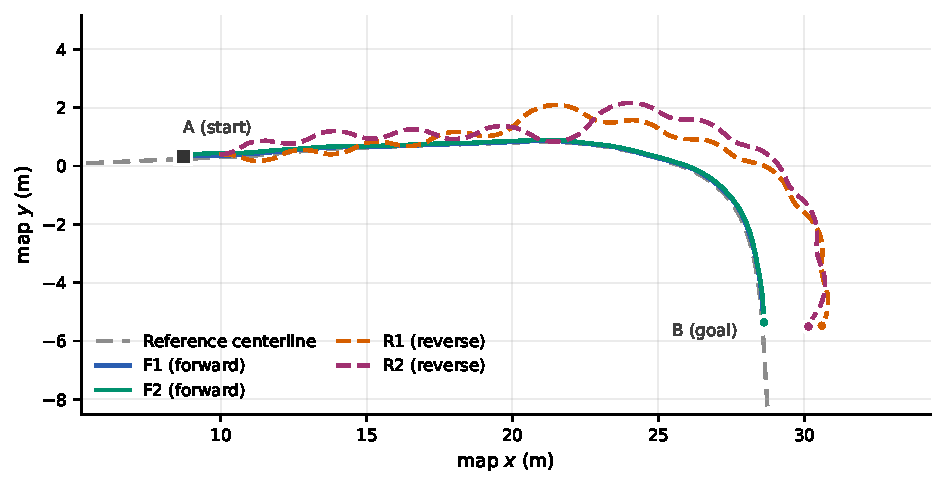
\includegraphics[width=0.9\textwidth]{figures/experiment_results/deployment_trajectories.pdf}
  \caption{Tractor tracks for the four successful deployment trials against the surveyed lane centerline. Solid tracks are forward trials, dashed tracks are reverse. The two forward tracks are nearly coincident and largely hide one another. The forward trials sit on the reference lane throughout, while the reverse trials bow outward by up to two meters before converging near point B.}
  \label{fig:deployment_trajectories}
\end{figure}

Forward tracking transferred essentially intact. The tractor held a mean cross-track error of $0.045$ and $0.078$\,m across the two trials, with worst-case deviations of $0.10$ and $0.16$\,m, which is tracking at the scale of the localization noise rather than of the controller. The trailer followed at $0.22$ and $0.26$\,m mean error and never left the lane corridor in either trial. Mean heading error was $1.3^\circ$ for the tractor and $3.8$ to $4.0^\circ$ for the trailer. The two forward trials agree with each other closely enough that their tracks overlay in \cref{fig:deployment_trajectories}, so the behavior is repeatable and not a single lucky run. Almost all of the forward error is concentrated in the final curve, where the trailer error rises from a mean of $0.10$\,m over the first 18\,m to $0.60$\,m over the last 5\,m and articulation reaches $39^\circ$, which is the expected cost of cutting a corner rather than a tracking failure.

Reverse is where the transfer degrades. The trailer held a mean cross-track error of $0.69$ and $0.76$\,m with worst excursions near $1.9$\,m, roughly three times the forward figure, and spent $11$\% of the maneuver outside the $1.41$\,m lane corridor. The tractor error is larger still, at $0.96$ and $1.10$\,m mean against $2.39$ and $2.35$\,m peak, and is the one metric where the tractor is worse than the trailer. That inversion is the expected signature of a reverse policy rewarded on trailer placement, which will carry the tractor wide to put the trailer where the path wants it. Mean articulation is $21^\circ$ against $9^\circ$ forward, and peak articulation reaches $51.6^\circ$, still comfortably inside the $80^\circ$ operational limit and the $90^\circ$ jackknife condition.

\subsection{Articulation Limit Cycle}
\label{sec:deployment_limit_cycle}

The difference between the two directions is not simply that reverse tracks less accurately. It is that the reverse trials exhibit a behavior the forward trials do not show at all, and that simulation does not reproduce: a sustained oscillation in the articulation angle. \Cref{fig:deployment_tracking} makes the contrast plain. In the forward trials the articulation trace is smooth and drifts slowly, moving off zero only for the final curve. In the reverse trials the hitch angle swings back and forth continuously, with a median peak-to-peak amplitude of $44$ to $46^\circ$ and a spatial wavelength of $2.4$ to $2.6$\,m, roughly one trailer length per cycle, sustained from the start of the maneuver to the end.

The third panel identifies the mechanism and rules out the obvious alternative explanations. In the forward trials the commanded steering rate never once reaches its $0.436$\,rad/s saturation limit. In the reverse trials it sits on that limit for $79$ to $80$\% of the control ticks, so the reverse policy is not regulating articulation smoothly but bang-banging the steering between its rate limits. Since both directions run on the same vehicle, the same actuator, the same articulation estimator, and the same bridge on the same day, neither the hardware nor the sensing can by itself account for the difference. What differs is the plant. Forward articulation dynamics are self-stabilizing, so estimate noise and actuation lag are damped out, while reverse articulation dynamics are unstable and the same disturbances are amplified into the limit cycle.

\begin{figure}[!tb]
  \centering
  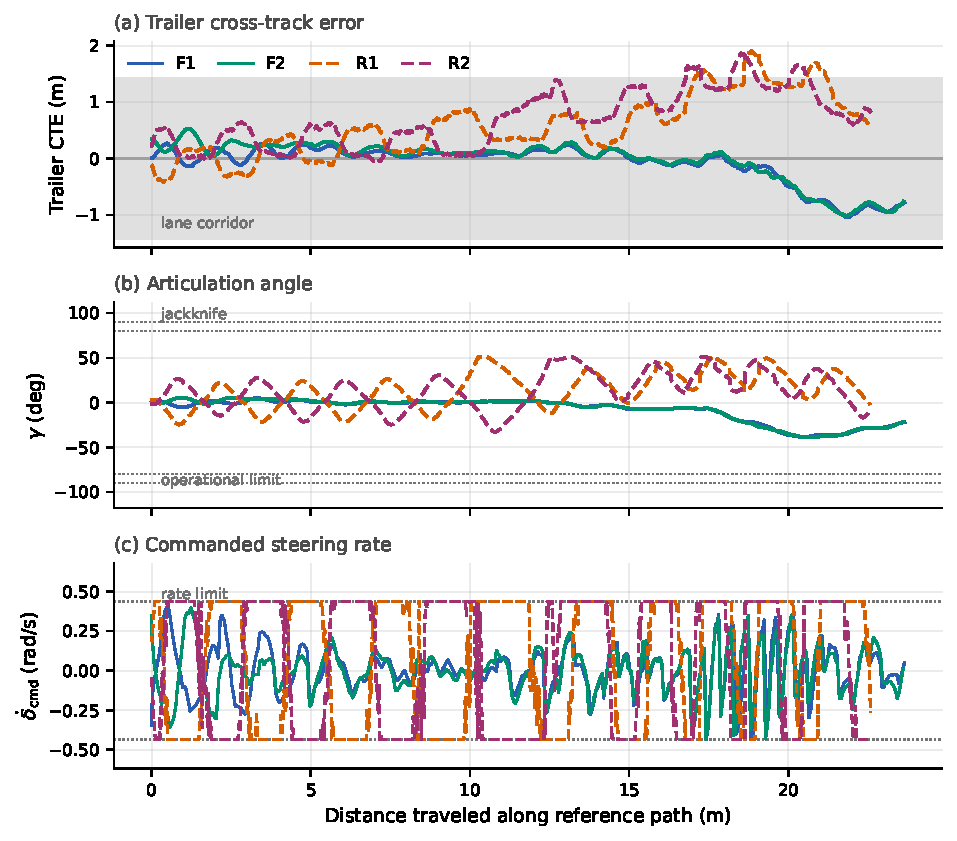
\includegraphics[width=0.88\textwidth]{figures/experiment_results/deployment_tracking.pdf}
  \caption{The four successful deployment trials against distance traveled along the reference path. (a) Trailer cross-track error, with the lane corridor shaded. (b) Articulation angle against the operational and jackknife limits. (c) Commanded steering rate against its saturation limit. Solid traces are forward trials, dashed traces are reverse. The reverse trials oscillate continuously and hold the steering rate on its limit, while the forward trials do neither.}
  \label{fig:deployment_tracking}
\end{figure}

This is the behavior expected of a delay-free-trained policy driving a lagging actuator, and it is the residue of the gap identified in \cref{sec:gap_actuation}. The Smith predictor removes enough of the loop delay that the vehicle remains stable and no trial jackknifed, but it does not remove all of it, and on the unstable reverse plant what is left closes a bang-bang limit cycle rather than settling. Articulation-estimate noise from the LiDAR rectangle fit of \cref{sec:gap_hitch} contributes on the same terms, since the policy acts on a noisy $\gamma$ at every tick. That both effects are invisible in the forward trials is consistent with this reading rather than an argument against it, because forward articulation dynamics damp exactly the disturbances that reverse dynamics amplify.

On a straight lane the limit cycle is largely benign, since the oscillation is symmetric and averages out, and the reverse trials hold the trailer inside the lane corridor through the straight section. It stops being benign at the curve, where the policy must hold a sustained articulation offset rather than swing around zero while having already spent most of its steering-rate authority on the oscillation. This is also where the four reverse trials excluded in \cref{sec:deployment_protocol} were ended. Each tracked the straight section normally for 11 to 13\,m, then lost the trailer outward as the lane began to curve, reaching trailer errors between $3.9$ and $4.2$\,m before the operator intervened. The reference curvature at that point saturates the $0.3$\,m$^{-1}$ clip applied to the curvature observation, so the policy also loses the ability to distinguish the sharpest part of the turn from a merely tight one exactly where it most needs to anticipate. Reverse tracking on this route is therefore best described as succeeding on the straight and marginal at the curve, with the margin decided by where in its oscillation cycle the vehicle happens to enter the turn.

\subsection{Comparison with Simulation}

The simulation benchmarks of \cref{tab:benchmark_forward,tab:benchmark_reverse} give the learned policy a $0.463$\,m mean trailer cross-track error forward and $0.935$\,m in reverse, with peak articulation of $8.2^\circ$ and $12.3^\circ$. Those distances are not directly comparable to the hardware figures, because the simulated vehicle is at Tesla Model S scale with a $10$\,m trailer while the laboratory platform carries a $2.8$\,m trailer. Normalized by trailer length, the simulated policy tracks to $0.046$ trailer lengths forward and the deployed policy to $0.087$, and in reverse to $0.094$ against $0.26$. Forward transfer therefore costs roughly a factor of two in relative tracking error, and reverse transfer roughly a factor of three.

The articulation comparison is the more informative one, because it is a pure angle and needs no scale correction. Forward peaks at $8.2^\circ$ in simulation and $39^\circ$ on hardware, but that excursion is confined to the final curve and the trace is otherwise smooth. Reverse peaks at $12.3^\circ$ in simulation and $51.6^\circ$ on hardware, and unlike the forward case the hardware trace oscillates for the entire maneuver. Simulation reproduces nothing resembling the limit cycle of \cref{fig:deployment_tracking} in either direction.

Taken together the two directions localize the sim-to-real gap more sharply than either could alone. The forward trials transfer at near-simulation quality on the same vehicle, the same actuator, the same estimator, and the same bridge that the reverse trials use, which rules out the vehicle model, the observation definitions, the action interface, and the bridge implementation as the source of the reverse degradation. What is left is the interaction between the residual actuation lag and articulation-estimate noise, both anticipated by \cref{sec:gap_actuation,sec:gap_hitch}, and the open-loop instability of reverse articulation dynamics that turns those small imperfections into a sustained oscillation. The deployment data now quantifies what that interaction costs.

What these trials establish should be read narrowly. They show that policies trained entirely in the 2D simulator drive a physical articulated vehicle along a real surveyed lane, at a scale and with a trailer geometry never seen in training and without any retraining on hardware, and that forward lane following transfers at a quality close to simulation. They do not establish reverse tracking at a quality suitable for unsupervised operation, and with two trials per direction they cannot characterize a completion rate. Closing the remaining gap is a matter of modeling the actuator lag and the articulation-estimate noise during training rather than compensating for them at deployment, which is taken up in \cref{ch:conclusion}.

\section{Summary}

This chapter demonstrated that the tractor-trailer control architecture developed in simulation can be ported to a physical platform by executing the trained RL policies directly through a bridging layer, rather than by re-deriving an analytical controller on the vehicle. The deployment retains Autoware's standard localization and perception augmented with the infrastructure sensor node obstacle list while replacing planning and control with an RL bridge that runs the forward and reverse policies at 10\,Hz over the same observation and action interfaces used in training. The principal engineering contributions are this RL bridge and its integration into a stripped-down Autoware stack, the onboard LiDAR hitch-angle estimator that recovers the articulation angle by rectangle fitting and Kalman filtering without any trailer-mounted sensor, and the Smith-predictor compensator that reconciles delay-free-trained policies with a lagging physical actuator. The gap analysis confirms that the simulation captures the dominant dynamics relevant to controller design, while identifying actuation delay, hitch-angle sensing, path-distribution mismatch, and localization reliability as the primary points of divergence between the simulated and physical systems. The deployment trials of \cref{sec:deployment_results} bear this out and sharpen it. Forward lane following transferred at close to simulation quality, holding the tractor within $0.16$\,m of the reference lane without any retraining, which shows that the vehicle model, the observation definitions, and the action interface all carried across correctly. Reverse ran on that same validated stack and degraded, sustaining a bang-bang articulation limit cycle that simulation does not exhibit and that leaves the maneuver marginal wherever the lane curves. The two gaps the analysis flagged first, actuation delay and articulation sensing, are therefore also the two that now limit deployed performance, and they bite only where the plant is open-loop unstable. Finally, the infrastructure sensor nodes, implemented and running in the laboratory, provide a route to occlusion-resilient perception behind the trailer without adding sensors to the trailer itself.
